% !TEX root = thesis.tex
\documentclass[thesis]{subfiles}

\begin{document}
%*******************************************************************************
%****************************** Second Chapter *********************************
%*******************************************************************************
\chapter{Background}
\label{background}
\begin{chapquote}{Mozer \etal, \textit{Using Relevance to Reduce Network Size Automatically, 1989}}
    ``One thing that connectionist networks have in common with brains is that if you open them up and peer inside, all you can see is a big pile of goo\href{https://yani.io/thesiseasteregg.html}{.}''
\end{chapquote}
Somewhat like their biologically inspiration, artificial neural networks (or simply \emph{neural networks}\index{neural network}) are easier to understand at the low-level --- the individual neuron itself lacks in complexity --- it is in the whole that it becomes hard to understand. While we will focus on the latter in the remainder of this dissertation, here we will present the basics behind the structure and training of neural networks and contemporary \glspl{dnn}\index{DNN}.

\section{Neural Networks}
Neural networks\index{neural network|textbf} are a broad range of statistical models characterized by consisting of a set of inter-connected nodes with non-linear \emph{activation functions} with learnable parameters, or \emph{weights}.
%, used in regression and classification problems.
 Although initially biologically inspired, neural networks within the field of machine learning have moved away from biologically-plausible models and towards entirely practical models guided by empirical results. Neural networks\index{neural network} are now the most popular statistical model used for learning applications in a diverse set of fields including computer vision, speech recognition, and medical imagery. 

We will not cover the long and colourful history of neural networks\index{neural network} (for this we recommend reading the introduction of \citet{goodfellow2016deep}), but attempt to instead provide the foundations, and thereafter an overview of contemporary models and methods directly relevant to this work. For a comprehensive overview of the basics of neural networks\index{neural network} we refer the reader to the excellent reference of \citet{Bishop1995}, and for a more recent  in-depth overview of the field of \emph{deep learning}, we refer the reader to \citet{goodfellow2016deep}. 

\subsection{The Neuron}
\begin{figure}[tbp]
\centering
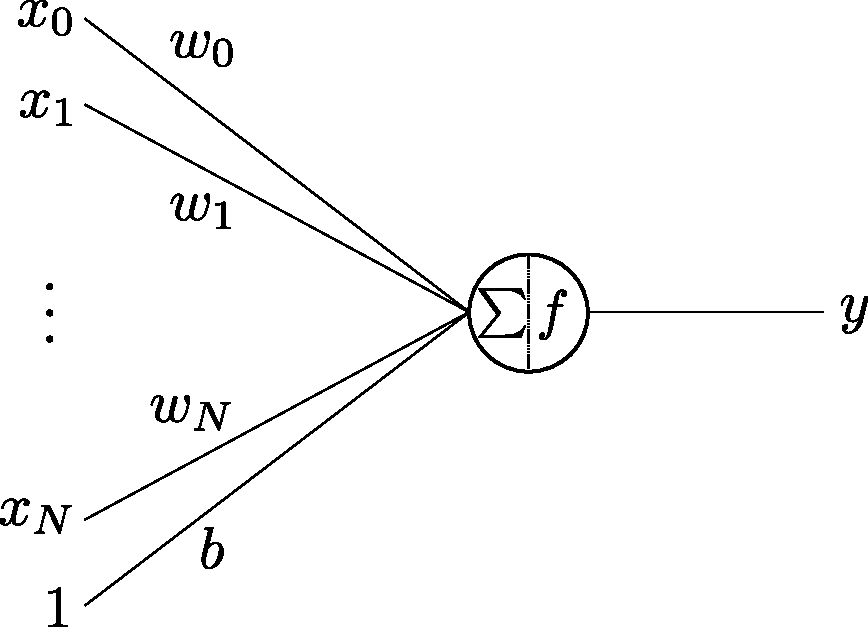
\includegraphics[width=0.5\textwidth]{neuron}
\caption[An illustration of a typical artificial neural network neuron]{\textbf{An illustration of a typical artificial neural network \emph{neuron}.} The neuron\index{neuron} is composed of output $\gls{y}$, a set of inputs, $\{\gls{x}_0, \ldots, \gls{x}_N\}$, input weights $\{\gls{w}_0, \ldots, \gls{w}_N\}$, bias $\gls{b}$ and activation function $\gls{f}$. Here the bias $\gls{b}$ is considered the weight of a fixed unit input.}
\label{fig:neuron}
\end{figure}
A neuron\index{neuron|textbf} is a function of the weighted aggregation of its many inputs: $\left\{\gls{x}_0,\ldots,\gls{x}_N\right\}$,
%
\begin{equation}
	\gls{y} = \gls{f}\left(\sum_{i}^{N} \gls{w}_i \gls{x}_i + \gls{b}\right),
\end{equation}
%
where $\gls{w}_i$ is the weight of the input $\gls{x}_i$, $\gls{f}$ is an \emph{activation function}, and $\gls{b}$ is the \emph{bias}. This is usually expressed more simply in matrix notation, where each neuron\index{neuron} consists of an input vector $\gls{vectorx}=(x_0,\ldots,x_N)$, weights $\gls{vectorw}=(w_0,\ldots,w_N)$ and a bias $\gls{b}$, the output of which is, %The bias term can also be considered as the weight of an input with a fixed value of $1$, as illustrated in \cref{fig:neuron}.
%
\begin{equation}
    \gls{y} = \gls{f}\left(\gls{vectorw}^T\gls{vectorx} + \gls{b} \right).
\end{equation}
%
If we assume the function $f$ to be a variant of the Heaviside step function,
\begin{equation}
    \gls{f}(\gls{x}) = 
\begin{cases}
1 & \text{if } \gls{x} \geq 0\\
0 \textrm{ (or $-1$)} & \text{if } \gls{x} < 0,
\end{cases}
\end{equation}
%
\begin{figure}[tbp]
\centering
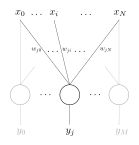
\includegraphics[width=0.5\textwidth]{singlelayer}
\caption[A single-layer neural network]{\textbf{An illustration of a simple single-layer neural network, such as a perceptron network.}}
\label{fig:singlelayer}
\end{figure}
then the neuron\index{neuron} is also called a \emph{perceptron}\index{perceptron|textbf}, a simple binary classifier, and one of the earliest connectionist learning methods, invented by \citet{rosenblatt1958perceptron} in 1957. A perceptron\index{perceptron} network is a single-layer neural network\index{neural network} (\ie a linear classifier), such as that illustrated in \cref{fig:singlelayer}, and should not to be confused with a \glsfmtfull{mlp} --- an unfortunate, but common, misnomer of any multi-layer neural network\index{neural network}.
\begin{figure}[tbp]
\centering
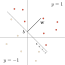
\includegraphics[width=0.5\textwidth]{perceptronline}
\caption[The interpretation of a perceptron\index{perceptron} as a hyperplane]{\textbf{The interpretation of a perceptron as a oriented hyperplane}, \ie a line, in $\mathbb{R}^2$.}
\label{fig:hyperplane}
\end{figure}
The perceptron\index{perceptron} also has a geometric interpretation~\citep{Bishop1995}, as shown in \cref{fig:hyperplane}. In 2D, for example, this is equivalent to the equation of the line. Assuming our perceptron\index{perceptron} only has a single input, \ie $N=1$, if we define $a\equiv \gls{w}_0$, $\gls{x} \equiv \gls{x}_0$, $c \equiv \gls{b}$, and $\gls{f}(\gls{x}) = \gls{x}$,
%
\begin{equation}
y = a x + c.
\end{equation}
%
In general a perceptron defines a \emph{hyperplane}, a separating manifold of dimension $d - 1$ for an input space of dimension $d$, a line in two dimensions, or plane in three dimensions. Neural networks are a discriminative classifier, and each neuron\index{neuron} can be visualized as a hyperplane functioning as a single decision boundary.

\subsection{The Limitations of Single-Layer Networks}\label{singlelayernetworks}
\begin{figure}[tbp]
\centering
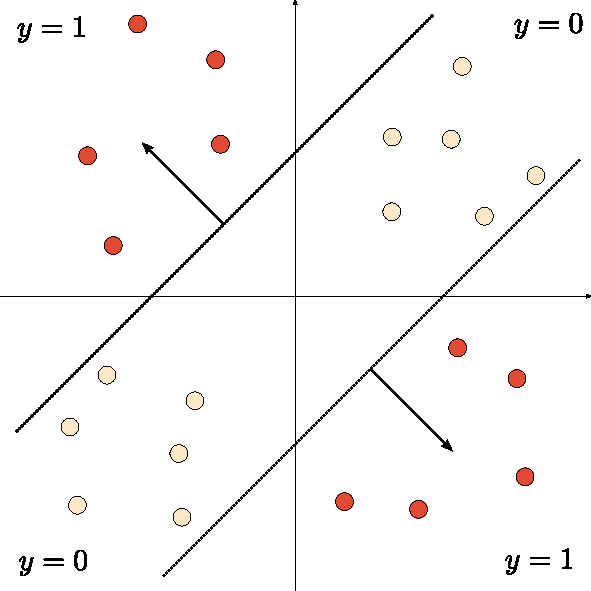
\includegraphics[width=0.5\textwidth]{perceptronxor}
\caption[An illustration of the inability to correctly classify the XOR function]{\textbf{An illustration of the inability of a single line (\ie a perceptron\index{perceptron}) to correctly classify the XOR function.} Instead, the composition of two lines is required to correctly separate these samples, \ie multiple layers.}
\label{fig:perceptronxor}
\end{figure}
A single-layer neural network\index{neural network}, such as the perceptron\index{perceptron}, is only a linear classifier, and as such is ineffective at learning a large variety of tasks. Most notably, in the 1969 book \emph{Perceptrons}~\citep{minsky1988perceptrons}, the authors showed that single-layer perceptrons\index{perceptron} could not learn to model functions as simple as the XOR function, amongst other non-linearly separable classification problems. As shown in \cref{fig:perceptronxor}, no single line can separate even a sparse sampling of the XOR function --- \ie\emph{it is not linearly separable}. Instead, only a composition of lines is able to correctly separate and classify this function, and other non-linearly separable problems.

At the time, it was not obvious how to train networks with more than one layer of neurons\index{neuron}, since the methods of learning neuron\index{neuron} weights, the \emph{perceptron learning rule}~\citep{rosenblatt1961principles} for perceptrons\index{perceptron} or the \emph{delta rule}\index{delta rule}~\citep{widrow1960adaptive} for general neurons\index{neuron}, only applied to single-layered networks. %This became known as the credit-assignment problem.

\subsection{Training Single Layer Networks: The Delta Rule}
\label{deltarule}
\begin{figure}[tbp]
\centering
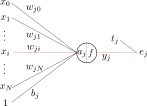
\includegraphics[width=0.5\textwidth]{neurononelayer}
\caption[Detailed illustration of a single-layer neural network]{\textbf{Detailed illustration of a single-layer neural network trainable with the delta rule\index{delta rule}.} The input layer consists of a set of inputs, $\{\gls{x}_{0}, \ldots, \gls{x}_{N}\}$. The layer has weights $\{\gls{w}_{j0}, \ldots, \gls{w}_{jN}\}$, bias $\gls{b}_j$, net neuron\index{neuron} activation $\gls{a}_j = \sum_i \gls{w}_{ji}$, activation function $\gls{f}$, and output $\gls{y}_j$. The error for output $\gls{y}_j$, $\gls{e}_j$, is calculated using the target label $\gls{t}_j$.}
\label{fig:neurononelayer}
\end{figure}

The delta rule\index{delta rule|textbf} for single-layered neural networks\index{neural network} is a gradient descent method, using the derivative of the network's weights with respect to the output error to adjust the weights to better classify training examples.

Training is performed on a training dataset $\gls{X}$, where each training sample $\gls{vectorx}^n\in \gls{X}$ is a vector $\gls{vectorx}^n = (\gls{x}^n_0, \ldots, \gls{x}^n_N)$. Assume that for a given training sample $\gls{vectorx}^n$, the $i$th neuron\index{neuron} in our single-layer neural network\index{neural network} has output $\gls{y}^n_j$, target (desired) output $t^n_j$, and weights $\gls{vectorw}=(\gls{w}_{j0}, \ldots, \gls{w}_{jM})$, as shown in \cref{fig:neurononelayer}. We can consider the bias to be an extra weight with a unit input, and thus we can omit the explicit bias from the derivation. 

We want to know how to change a given weight $\gls{w}_{ji}$ given the output of node $j$ for a given input data sample $\gls{vectorx}^n$, 
\begin{equation}
	\gls{y}^n_j = \gls{f}\left( \gls{a}^n_j \right),
	\label{eqn:output}
\end{equation}
where the net activation $\gls{a}^n_j$ is,
\begin{equation}
	\gls{a}^n_j = \sum_i \gls{w}_{ji} \gls{x}^n_{i}.
	\label{eqn:weightsum}
\end{equation}
To do so, we must use the error of our prediction for each output $\gls{y}_j$ and training sample $\gls{x}^n$ as compared to the known label $\gls{t}_j$,
\begin{equation}
    \gls{e}^n_j = \gls{y}^n_j - \gls{t}^n_j.
    \label{eqn:error}
\end{equation}
%
For this derivation, we assume the error for a single sample is calculated by the sum of squared errors of each output. In fact, the derivation holds as long as our error function is in the form of an average~\citep{Bishop1995},
\begin{equation}
    \gls{E}^n = \frac{1}{2} \sum_j {\left(\gls{e}^n_j\right)}^2.
    \label{eqn:errorsum}
\end{equation}
Chain rule allows us to calculate the \emph{sensitivity} of the error to each weight $\gls{w}_{ji}$ in the network,
\begin{equation}
\begin{aligned}
    \frac{\partial \gls{E}^n}{\partial \gls{w}_{ji}} &= \frac{\partial \gls{E}^n}{\partial \gls{e}^n_j}\frac{\partial \gls{e}^n_j}{\partial \gls{y}^n_j} \frac{\partial \gls{y}^n_j}{\partial \gls{a}^n_j} \frac{\partial \gls{a}^n_j}{\partial \gls{w}_{ji}}.
\end{aligned}
\end{equation}
%
Differentiating \cref{eqn:errorsum} with respect to $\gls{e}^n_j$,
\begin{equation}
\begin{aligned}
    \frac{\partial \gls{E}^n}{\partial \gls{e}^n_j} &= \gls{e}^n_j,
\end{aligned}
\end{equation}
%
\cref{eqn:error} with respect to $\gls{y}^n_j$,
\begin{equation}
\begin{aligned}
    \frac{\partial \gls{e}^n_j}{\partial \gls{y}^n_j} &= 1,
\end{aligned}
\end{equation}
%
\cref{eqn:output} with respect to $\gls{a}^n_j$,
\begin{equation}
\begin{aligned}
   \frac{\partial \gls{y}^n_j}{\partial \gls{a}^n_j}  &= \gls{f}'\left( \gls{a}^n_j \right),
\end{aligned}
\label{eqn:partialdyda}
\end{equation}
%
and finally \cref{eqn:weightsum} with respect to $\gls{w}_{ji}$,
\begin{equation}
\begin{aligned}
   \frac{\partial \gls{a}^n_j}{\partial \gls{w}_{ji}} &= \frac{\partial}{\partial \gls{w}_{ji}} \left( \sum_i \gls{w}_{ji} \gls{x}_{i} \right)\\
   &= \gls{x}_i,
\end{aligned}
\label{eqn:sumonetermpartial}
\end{equation}
since only one of the terms in the sum is related to the specific weight $\gls{w}_{ji}$. Thus the sensitivity is,
\begin{equation}
\label{eqn:deltasensitivity}
\begin{aligned}
    \frac{\partial \gls{E}^n}{\partial \gls{w}_{ji}} &= \gls{e}^n_j  \gls{f}'\left( \gls{a}^n_j \right) \gls{x}_i.
\end{aligned}
\end{equation}
%
Typically what is variously called the local gradient, error, or simply \emph{delta}, is then defined,
\begin{equation}
\label{eqn:delta}
\begin{aligned}
    \gls{delta}^n_j &\equiv \frac{\partial \gls{E}^n}{\partial \gls{a}^n_j}\\
    &= \frac{\partial \gls{E}^n}{\partial \gls{e}^n_j}\frac{\partial \gls{e}^n_j}{\partial \gls{y}^n_j} \frac{\partial \gls{y}^n_j}{\partial \gls{a}^n_j}\\
    &= e^n_j  \gls{f}'\left( a^n_j \right),
\end{aligned}
\end{equation}
%
such that \cref{eqn:deltasensitivity} can be rewritten,
\begin{equation}
\begin{aligned}
    \frac{\partial \gls{E}^n}{\partial \gls{w}_{ji}} &= \gls{delta}^n_j \gls{x}_i.
\end{aligned}
\end{equation}
%
The delta rule\index{delta rule} adjusts each weight $\gls{w}_{ji}$ proportional to the sensitivity, 
\begin{equation}
\begin{aligned}
    \Delta \gls{w}_{ji} &= -\gls{lr} \frac{\partial \gls{E}^n}{\partial \gls{w}_{ji}},
\end{aligned}
\end{equation}
%
where $\gls{lr}$ is a constant called the \emph{learning rate} or \emph{step size}. Using the delta defined in \cref{eqn:delta}, this is simply written,
\begin{equation}
\begin{aligned}
    \Delta \gls{w}_{ji} &= -\gls{lr} \gls{delta}^n_j x_i.
\end{aligned}
\end{equation}
%
\subsection{Backpropagation}
The credit-assignment problem was solved with the discovery of \emph{backpropagation}\index{backpropagation|textbf} (also known as the \emph{generalized delta rule}), allowing learning in multi-layer neural networks\index{neural network}. It is somewhat controversial as to who first `discovered' backpropagation\index{backpropagation}, since it is essentially the application of the chain rule to neural networks\index{neural network}, however it's generally accepted that it was first demonstrated experimentally by \citet{rumelhartbackprop}. Although it is ``just the chain rule'', to dismiss this first demonstration of backpropagation\index{backpropagation} in neural networks\index{neural network} is to understate the importance of this discovery to the field, and to dismiss the practical difficulties in first implementing the algorithm --- a fact that will be attested to by anyone who has since attempted.

The following is a derivation of backpropagation\index{backpropagation} loosely based on the excellent references of \citet{haykin1994neural,Bishop1995}, although with different notation. This derivation builds upon the derivation for the delta rule\index{delta rule} in the previous section, although it is important to note that, as shown in \cref{fig:neurontwolayer}, the indexing we will use to refer to neurons\index{neuron} of different layers differs from that in \cref{fig:neurononelayer} for the single-layer case.

We are interested in finding the sensitivity of the error $\gls{E}$ to a given weight in the network $\gls{w}_{ij}$. There are two classes of weights for which we must derive different rules, 
\begin{enumerate*}[label= (\textbf{\roman*})]
  \item\label{enum:outputneuron} those belonging to \emph{output layer neurons\index{neuron}}, \ie neurons\index{neuron} lying directly before the output, such as $\gls{w}_{kj}$ in \cref{fig:neurontwolayer}, and
  \item\label{enum:hiddenneuron} weights belonging to hidden layer neurons\index{neuron}, such as $\gls{w}_{ji}$ in \cref{fig:neurontwolayer}.
\end{enumerate*}
%
\paragraph{\ref{enum:outputneuron}~Output Layer}
The output weights are relatively easy to find, since they correspond to the same types of weights found in single-layer networks, and have direct access to the error signal, \ie$\gls{e}^n_j$. Indeed the derivation in \cref{deltarule} also describes the sensitivity of the weights in the output layer of a multi-layer neural network\index{neural network}. With some change of notation (now indexing by $k$ rather than $j$ to match \cref{fig:neurontwolayer}), we can use the sensitivity found in \cref{eqn:deltasensitivity},
%
\begin{equation}
\begin{aligned}
    \frac{\partial \gls{E}^n}{\partial \gls{w}_{kj}} &= \frac{\partial \gls{E}^n}{\partial \gls{a}^n_k} \frac{\partial \gls{a}^n_k}{\partial \gls{w}_{kj}}\\
%    \frac{\partial E^n}{\partial w_{kj}} &= \frac{\partial E^n}{\partial e^n_k}\frac{\partial e^n_k}{\partial y^n_k} \frac{\partial y^n_k}{\partial a^n_k}\\
%    &= - e^n_k  \gls{f}'\left( a^n_k \right) x^n_{kj}\\
    &= \gls{delta}^n_k \gls{x}^n_{kj}\\
    &= \gls{delta}^n_k \gls{y}^n_j.
\end{aligned}
\label{eqn:outputlayer}
\end{equation}
%
\paragraph{\ref{enum:hiddenneuron} Hidden Layer}
\begin{figure}[tbp]
\centering
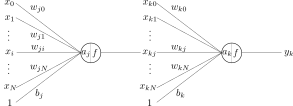
\includegraphics[width=0.8\textwidth]{neurontwolayer}
\caption[Detailed illustration of a neural network with a single hidden layer]{\textbf{Detailed illustration of a neural network with a single hidden layer.} The input layer consists of a set of inputs, $\{\gls{x}_{0}, \ldots, \gls{x}_{N}\}$. The hidden layer has weights $\{\gls{w}_{i0}, \ldots, \gls{w}_{iN}\}$, bias $\gls{b}_i$, net neuron\index{neuron} activity $\gls{a}_j = \sum_i \gls{w}_{ji}$ and activation function $\gls{f}$. The output layer with output $\gls{y}_k$, has weights $\{\gls{w}_{k0}, \ldots, \gls{w}_{jN}\}$ and bias $\gls{b}_j$. The error for output $\gls{y}_k$, $\gls{e}_k$, is calculated using the target label $\gls{t}_k$. Note that $\gls{x}^n_{kj} \equiv \gls{y}^n_j$.}
\label{fig:neurontwolayer}
\end{figure}
We will first derive the partial derivative ${\partial \gls{E}^n}/{\partial \gls{w}_{ji}}$, for a single hidden layer network, such as that illustrated in \cref{fig:neurontwolayer}. Unlike in the first case, the weights belonging to hidden neurons\index{neuron} have no direct access to the error signal, instead we must calculate the error signal from all of the neurons that indirectly connect the neuron\index{neuron} to the error (\ie every output neuron\index{neuron} $\gls{y}_k$).

Following from the chain rule we can write the partial derivative of a hidden weight $\gls{w}_{ji}$ with respect to the error $\gls{E}^n$,
\begin{equation}
\begin{aligned}
    \frac{\partial \gls{E}^n}{\partial \gls{w}_{ji}} &= \underbrace{\left( \sum_k \frac{\partial \gls{E}^n}{\partial \gls{e}^n_{k}}
     \frac{\partial \gls{e}^n_{k}}{\partial \gls{y}^n_{k}} \frac{\partial \gls{y}^n_{k}}{\partial \gls{a}^n_k} \frac{\partial \gls{a}^n_k}{\partial \gls{y}^n_{j}}\right)}_\text{output neurons}
     \underbrace{\frac{\partial \gls{y}^n_{j}}{\partial \gls{a}^n_{j}} \frac{\partial \gls{a}^n_{j}}{\partial \gls{w}_{ji}}}_\text{hidden neuron},
     \label{eqn:twolayer1}
\end{aligned}
\end{equation}
%
where the sum arises from the fact that, unlike in \cref{eqn:sumonetermpartial} where the weight $\gls{w}_{kj}$ affects only a single output, the hidden weight $\gls{w}_{ji}$ affects all neurons\index{neuron} in the subsequent layer (see \cref{fig:neurontwolayer}).

We already know how to calculate the partials for the output layer from the derivation of the delta rule\index{delta rule} for single-layer networks, and we can substitute these from \cref{eqn:outputlayer} for the output neuron\index{neuron} and error partial derivatives,
%
\begin{equation}
\begin{aligned}
    \frac{\partial \gls{E}^n}{\partial \gls{w}_{ji}} &= \left( \sum_k \gls{delta}^n_k \gls{y}^n_j \frac{\partial \gls{a}^n_k}{\partial \gls{y}^n_{j}}\right)
     \frac{\partial \gls{y}^n_{j}}{\partial \gls{a}^n_{j}} \frac{\partial \gls{a}^n_{j}}{\partial \gls{w}_{ji}}.
     \label{eqn:twolayer2}
\end{aligned}
\end{equation}
%
Recall from \cref{eqn:weightsum}, the net activation $\gls{a}$ is a sum of all previous layer weights. Thus,
\begin{equation}
\begin{aligned}
    \frac{\partial \gls{a}^n_k}{\partial \gls{y}^n_{j}} &= \frac{\partial}{\partial \gls{y}^n_{j}}\left(\sum_j \gls{w}_{kj} \gls{y}^n_{j} \right) &= \gls{w}_{kj},
\end{aligned}
\end{equation}
%
and substituting from \cref{eqn:partialdyda} and \cref{eqn:sumonetermpartial} into \cref{eqn:twolayer2},
\begin{equation}
\begin{aligned}
    \frac{\partial \gls{E}^n}{\partial \gls{w}_{ji}} &= \left( \sum_k \gls{delta}^n_k \gls{y}^n_j \gls{w}_{kj}\right)
	\gls{f}'\left( \gls{a}^n_j \right) \gls{x}_i.
     \label{eqn:twolayer3}
\end{aligned}
\end{equation}
%
This bears some resemblance to the derived expression for a single-layer, and just as in \cref{eqn:delta}, we can use our definition of the delta to simplify it. For hidden layers this evaluates as
\begin{equation}
\label{eqn:deltahidden}
\begin{aligned}
    \gls{delta}^n_j &\equiv \frac{\partial \gls{E}^n}{\partial \gls{a}^n_k}\\
    &= \left( \sum_k \frac{\partial \gls{E}^n}{\partial \gls{e}^n_{k}} \frac{\partial \gls{e}^n_{k}}{\partial \gls{y}^n_{k}} \right) \frac{\partial \gls{y}^n_{k}}{\partial \gls{a}^n_k}\\
    &= \left(\sum_k \gls{delta}^n_k \gls{y}^n_j \gls{w}_{kj} \right) \gls{f}'\left( \gls{a}^n_j \right).
\end{aligned}
\end{equation}
%
This leaves us with the more convenient expression (as we will see in \cref{arbitraryhidden}),
\begin{equation}
\begin{aligned}
    \frac{\partial \gls{E}^n}{\partial \gls{w}_{ji}} &=  \gls{delta}^n_j \gls{x}_i.
     \label{eqn:twolayer4}
\end{aligned}
\end{equation}
%
\subsubsection{Arbitrary Number of Hidden Layers}
\label{arbitraryhidden}
The derivation above was based on the specific case of a single hidden layer network, but it is trivial to extend this result to multiple hidden layers. There is a recursion in the calculation of the partial derivatives in \cref{eqn:deltahidden} which holds for a network with any number of hidden layers, and which we will now make explicit. 

The delta is defined,
\begin{equation}
\gls{delta}^n_i = \begin{cases}
        \gls{f}'\left( \gls{a}^n_j \right) \gls{e}^n_j \,& \textrm{when neuron\index{neuron} $j$ is output}\\
        \gls{f}'\left( \gls{a}^n_j \right) \left( \sum_j \gls{delta}^n_j \gls{y}^n_i \gls{w}_{ji} \right)& \textrm{when neuron\index{neuron} $j$ is hidden},
        \end{cases}
\label{eqn:fulldeltadefinition}
\end{equation}
for any adjacent neural network\index{neural network} layers $i, j$, including the output layer where the outputs are considered to have an index $j$. The sensitivity is then, 
\begin{equation}
\begin{aligned}
    \frac{\partial \gls{E}^n}{\partial \gls{w}_{ji}} &=  \gls{delta}^n_j y_i.
     \label{eqn:sensitivity}
\end{aligned}
\end{equation}
%
\subsection{Learning with Backpropagation}
Learning with backpropagation\index{backpropagation} is much like the delta rule\index{delta rule}; sensitivities are used to correct weights proportional to a constant \emph{learning rate} or \emph{step size} parameter $\gls{lr}$. Although the correction is proportional to the sensitivity, we wish to \emph{reduce} the error $E^n$, and so we move the weight in the opposite direction of the gradient~\footnote{Note that, rather than optimizing the error function directly, usually a surrogate loss that is easier to optimize is used, \eg negative log-likelihood for classification.}. Formally, the weight change rule is given by,
\begin{equation}
\begin{aligned}
    \Delta \gls{w}^n_{ij} &= -\gls{lr} \frac{\partial \gls{E}^n}{\partial \gls{w}_{ji}}\\
    &= -\gls{lr} \, \gls{delta}^n_j \gls{y}_i,
     \label{eqn:backproplearningrule}
\end{aligned}
\end{equation}
where $\gls{delta}^n_j$ is as defined in \cref{eqn:fulldeltadefinition}, and $y_i$ is the output of neuron\index{neuron} $i$.
%
\begin{figure}[tbp]
\centering
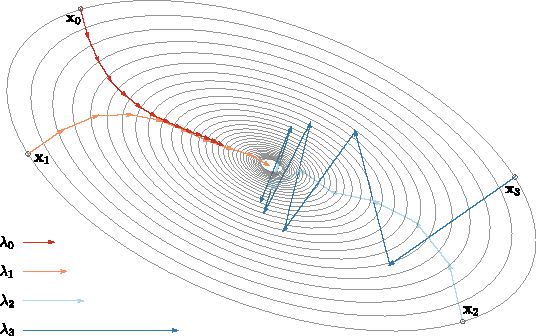
\includegraphics[width=0.85\textwidth]{learningratedecrease}
\caption[Learning rate and convergence]{\textbf{An illustration of the effect of step size (learning rate) and learning policy on convergence with backpropagation\index{backpropagation}.} This example is of a symmetric 2D error surface, where the parameters are initialized to one of the symmetrically identical surface points $x_i$ where $i=0\ldots4$. For each of the different initial learning rates $\gls{lr}_i$, the learning rate is decreased by $10\%$ each iteration.}\label{fig:learningrate}
\end{figure}
Backpropagation\index{backpropagation} is a method of steepest descent. This is illustrated in \cref{fig:learningrate}, where the backpropagation\index{backpropagation} learning rule, \cref{eqn:backproplearningrule}, specifies a step size in the form of the \emph{learning rate}. The learning rate parameter scales the step size, or the magnitude of the weight change vector. \Cref{fig:learningrate} also illustrates the effect of learning rate on gradient descent. Too small a learning rate can result in very slow learning such as for $\gls{lr}_0$, while too large a step size can result in bouncing around the minima ($\gls{lr}_2, \gls{lr}_3$), or missing it altogether. 

In order to settle into a local minima, the learning rate must also be decreased as training progresses. However, too fast a rate of decrease and it may never reach the basin of attraction of the local minima, as with $\gls{lr}_0$, while if the rate of decrease is too slow it will take a very long time to enter the basin of attraction, such as with $\gls{lr}_3$. 

The balance of trying to find an appropriate learning rate and learning policy is unfortunately part of the `black magic' behind training \glspl{dnn}\index{DNN} which comes from experience, but \citet{Bottou2012sgdtricks, goodfellow2016deep} are excellent references on some of the common approaches taken to make this task simpler.

\subsection{The Problem with First-Order Optimization}\label{pathological}
The underlying reason learning rate and learning policy has such a large effect is that gradient descent is a \emph{first-order} optimization method, and only considers the first-order partial derivatives, \ie for a 2D error surface $\gls{E}(x, y)$, gradient descent moves in the opposite direction of the gradient,
\begin{equation}
    \nabla \gls{E}(x, y) = {\left(\frac{\partial \gls{E}}{\partial \gls{x}}, \frac{\partial \gls{E}}{\partial \gls{y}}\right)}.
\end{equation}
This gradient tells us the direction of maximum increase at a given point on the error surface, but it does not tell us any information about the \emph{curvature} of the surface at that point. The curvature of the surface is described by higher-order derivatives such as the second-order partial derivatives, \eg
%\begin{equation}
	$\pd[2]{E}{x}$,
%\end{equation}
and mixed partial derivatives, \eg
%\begin{equation}
	$\md{E}{2}{x}{2}{y}{2}$.
%\end{equation}
%
\begin{figure}[tbp]
\centering
\begin{subfigure}[b]{0.45\textwidth}
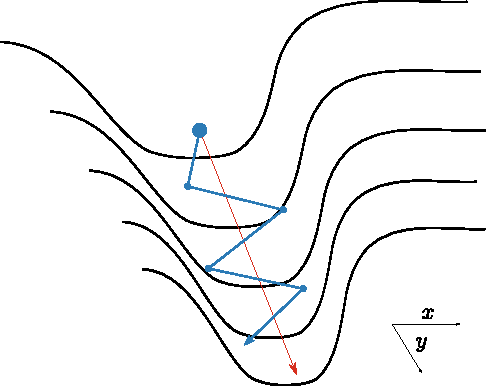
\includegraphics[width=\textwidth]{narrowvalley}
\caption{Gradient descent}\label{fig:narrowvalleysgd}
\end{subfigure}
\begin{subfigure}[b]{0.45\textwidth}
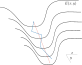
\includegraphics[width=\textwidth]{narrowvalleymomentum}
\caption{Momentum}\label{fig:narrowvalleymomentum}
\end{subfigure}
\caption[Pathological curvature]{\textbf{Pathological curvature.} An error surface $\gls{E}(x, y)$ exhibiting a narrow valley, and the optimal path from the starting point to the minima shown by the red arrow. In a pathological error surface such as this, first-order methods cannot use the information provided by the Hessian\index{Hessian} on the surface curvature to avoid bouncing along the walls of the valley, slowing descent. Momentum alleviates this somewhat in damping the change in direction, by preserving information on previous gradients, allowing a quicker descent. Inspired by a similar diagram by \citet{martens2010deep}.}
\label{fig:pathological}
\end{figure}
These second-order partials give important information about the curvature of the error surface $\gls{E}$. For example, in \cref{fig:learningrate}, the error surface takes on an elliptical shape, which causes problems when we only consider the direction of maximum decrease $-\nabla \gls{E}$. The classic example of such a pathological error surface for first-order methods is an error surface that looks like a narrow valley, as shown in \cref{fig:narrowvalleysgd}. With an initialization outside the bottom of the valley, gradient descent will bounce along the walls of the valley, leading to a very slow learning convergence.

For well-behaved surfaces where the scaling of parameters is similar
%, \ie surfaces where the mixed partial derivatives, \eg
%\begin{equation}
%    \frac{\partial^2 E}{\partial x\,\partial y} \approx 1,
%\end{equation}
basins of attraction around a minima are roughly circular, and thus avoid this problem, since the first-order gradients will point almost directly at the minima for any location on the error surface.

There are second-order optimization methods based on Newton's method, however the issue is that they do not scale to the size of any practical \glspl{dnn}\index{DNN}. The matrix of second-order partial derivatives for a scalar-values function, the Hessian\index{Hessian} $\gls{hessian}$, is required for any full second-order optimization method, however the Hessian\index{Hessian} is square in the number of parameters in the network. For networks of millions of parameters this means storing the Hessian\index{Hessian} is infeasible.

There are a whole slew of optimization tricks for gradient descent, often attempting to compensate for the shortcomings of first-order optimization without using the Hessian\index{Hessian}, or using some approximation to it. We will not cover those here, since none of these were used in our experiments. A full background of the issues of optimization in \glspl{dnn}\index{DNN} is outside the scope of this dissertation, however interested readers should refer to \citet{goodfellow2016deep} to learn more about these methods, and \citet{martens2010deep} for an excellent introduction to the problems of first and second-order optimization in \glspl{dnn}\index{DNN}.

\subsection{Momentum}
A common improvement to gradient descent is momentum~\citep{polyak1964some,rumelhartbackprop}, a trick for minimizing the effect of pathological curvature on gradient descent, which also helps with variance in gradients. The name comes from the analogy of the update to physical momentum $\rho$ for a moving particle, $\mathbf{p}=m\gls{velocity}$, where we assume unit mass, $m=1$.

In momentum, the gradients over multiple iterations are accumulated into a velocity gradient, 
\begin{equation}
\begin{aligned}
\gls{velocity}_{\gls{iteration}+1} &= \alpha \gls{velocity}_{\gls{iteration}} - \gls{lr}\nabla \gls{E}(\gls{vectorw})\\
\Delta\gls{vectorw} &= \gls{vectorw}_t + \gls{velocity}_{\gls{iteration}+1},
\end{aligned}
\end{equation}
where $\gls{lr}$ is the learning rate, $\gls{iteration}$ is the iteration,  $\nabla \gls{E}$ is the gradient of the error surface $\gls{E}(\gls{vectorw})$ being minimized, and $\gls{vectorw}$ is the weight vector optimized. Momentum in effect stores some information on the gradients found in past iterations, and uses this to damp the effect of a new gradient on the search direction, as illustrated in \cref{fig:narrowvalleymomentum}. For error surfaces with pathological curvatures, this can dramatically speed up learning.

\subsection{Online, Batch and Stochastic Gradient Descent}
Although the backpropagation\index{backpropagation} weight change rule, \cref{eqn:backproplearningrule}, tells us how to change the weights given a single training sample $\gls{x}^n$, in practice this method is rarely used. The reason is simply that the gradients from a single sample are too biased, or noisy, and they are not representative of the dataset in general; $\Delta \gls{w}^n_{ij}$ is only an approximation to the true gradient we want --- it is only from one sample, $\gls{x}^n$, of the training dataset $\gls{X}$. 

\subsubsection{Batch Gradient Descent}
At the opposite end of the spectrum there is \emph{batch} training\index{batch training|textbf} where the gradient is computed over all data samples in the training set,
\begin{equation}
\begin{aligned}
    \Delta \gls{w}_{ij} &= -\gls{lr}\frac{1}{N} \sum^N_{n=0} \frac{\partial \gls{E}^n}{\partial \gls{w}_{ji}},
     \label{eqn:batchlearningrule}
\end{aligned}
\end{equation}
%
where $N$ is the number of training samples in $\gls{X}$. Batch training\index{batch training} gives us the true gradient, however it is also very expensive, since it requires us to perform the forward pass of the network over all training samples for every update. 

\subsubsection{Stochastic Gradient Descent}
Instead of computing the gradient on only one training sample, or over the entire training set, we might instead use a significant subset of the training set --- a \emph{mini-batch}. This approach is called \gls{sgd}.

When using \gls{sgd}, we randomly sample (without replacement) a subset of the training set $X_{\textrm{mb}} \subset \gls{X}$, such that
\begin{equation}
\begin{aligned}
    \Delta \gls{w}_{ij} &= -\gls{lr} \frac{1}{|X_{\textrm{mb}}|} \sum_{\{n|\,\gls{vectorx}^n \in \gls{X}_{\textrm{mb}}\}} \frac{\partial \gls{E}^n}{\partial \gls{w}_{ji}},
     \label{eqn:sgdrule}
\end{aligned}
\end{equation}
where the size of the mini-batch $|\gls{X}_{\textrm{mb}}|$ should be significant enough to represent the statistics of the training set distribution, \ie for a classification problem the mini-batch should capture a significant number of the classes in the training set. Using a mini-batch size of one, \ie a single sample as shown in \cref{eqn:backproplearningrule}, is a special case of \gls{sgd}. 

It has been observed in practice that adding noise to the gradient by using stochastic gradient descent often helps generalization compared to batch gradient descent, perhaps by preventing overfitting. Note that even if we use the true gradient for the training dataset, the training set $X$ is only a sampling of the population distribution we want our network to generalize to.

\subsection{Activation Functions}\label{activationfunctions}
As we have seen with the perceptron\index{perceptron}, the activation function for a single-layer network can provide a means of pushing the outputs of each neuron\index{neuron} towards a binary classification. However the activation function has a much more important function in multi-layer neural networks\index{neural network}. Without a non-linear activation function, even a large multi-layer neural network\index{neural network} would only have the representational power of a linear classifier --- the composition of linear functions is a linear function. For this reason, the \emph{activation function} $\gls{f}$ is a non-linear function applied to the output of a neuron\index{neuron} to allow multi-layer networks to learn complex non-linear functions,

\begin{equation}
\gls{y} = \gls{f}\left(\gls{vectorw}^T\gls{vectorx} + \gls{b}\right).
\end{equation}
%
In the field of neural networks\index{neural network}, activation functions have classically been chosen to be a \emph{sigmoid} function, \ie a function mapping negative inputs to negative outputs and positive inputs to positive outputs with a smooth transition around $\gls{a} = 0$. This is a nice property to have, since the function is still pushing the outputs of the network towards a binary classification, the function is non-linear (so composition of functions are non-trivial), and the function has well-defined gradients. Examples of sigmoid functions commonly used include the logistic function, 

\begin{equation}
	\gls{f}(\gls{a}) = \frac{1}{1+e^{-\gls{a}}},
\end{equation}
%
and they hyperbolic tangent,
\begin{equation}
	\gls{f}(\gls{a}) = \tanh(\gls{a}).
\end{equation}
%
An issue with sigmoidal activation functions however, is that the gradients are very small in a large part of the domain of the function. For this reason, and improved empirical results, modern neural networks\index{neural network} tend to use the \gls{relu} activation function, as described in \cref{section:relu}.


\subsection{Deep \Vs Shallow Neural Networks}
Neural networks with at least one (infinitely wide) \emph{hidden} layer have been proven to be a universal approximator --- \ie such a neural network\index{neural network} can theoretically represent any function~\citep{journals/mcss/Cybenko92,hornik89a}. This is in stark contrast to the limitations of neural networks\index{neural network} without hidden layers, as explained in \cref{singlelayernetworks}.

In practice however we do not find that a network with only a single hidden layer, of even a very large width, can learn to represent complex functions as well as networks with many hidden layers. Indeed the observation that networks with many hidden layers, or \emph{deep} networks, empirically achieve better accuracy than networks with few hidden layers, or \emph{shallow} networks, represents some of the progress made in learning with neural networks\index{neural network} in recent years. Unfortunately the reasons why this mismatch between theory and practice occurs is still poorly understood, and an active area of research.

\subsection{Convolutional Neural Networks}\label{cnns}
The earliest work on what are now termed \glspl{cnn}\index{CNN|textbf} was by \citeauthor{Fuk80}, on the \emph{Neocognitron}~\citep{Fuk80,fukushima2013artificial}. The Neocognitron was a biologically motivated architecture, motivated by what are typically called simple and complex cells in the primary visual cortex (V1). To model simple cells; cells whose response correlated with simple oriented edges in a translation invariant manner, the Neocognitron used shared weights which were connected to local image patches of the input image (and were not simply described as convolution of a filter). Complex cells were modelled by a ``blurring'' operation, what we now term more generally as \emph{pooling}. The Neocognitron network consisted of alternating layers of simple and complex cells, \ie alternating convolution and pooling layers, much as seen in state-of-the-art convolutional networks. In an era in which fully-connected networks were used to learn any input type \citeauthor{Fuk80} showed that for structured inputs a drastically different architecture could make a big difference in generalization. 

Despite the pioneering novelty of the work on Neocognitron, it was only following the simplification and improvement of \citet{Lecun1998} in both the description of the network and its operation that it gained wider acknowledgement as a breakthrough for image recognition. In their work the local shared weights of the Neocognitron are put in the context of convolution, and the averaging operation replaced with max-pooling. The application to handwritten digit recognition gave state-of-the-art results, and would result in the \emph{LeNet5} network, still used today in some commercial applications.

The application of the LeNet-style \gls{cnn} architecture to more complex problems, however, proved infeasible~\citep{goodfellow2016deep}. These problems required a deeper hierarchy of representation, which implied a large number of layers. Networks with a large number of layers proved to be un-trainable due to numerous issues with the model itself, notably vanishing gradients~\citep{hochreiter1991untersuchungen}, and the lack of large datasets and computational power at the time. Convolutional neural networks\index{neural network} fell out of favour, and were passed over in favour of the more successful paradigm of using hand-crafted local features, such as \gls{sift}~\citep{Lowe2004} for many tasks, and in particular the problem of \gls{objectinstancerecognition} was well addressed by such solutions. Meanwhile \gls{objectclassrecognition} remained a difficult problem, for which the best solutions were deformable parts models, also based on local features.

\subsubsection{Convolutional Layers}
\begin{figure}[tb]
	\centering
	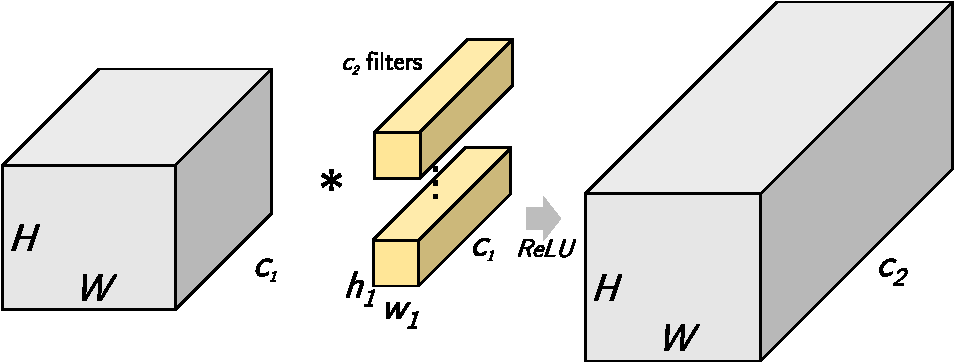
\includegraphics[width=0.66\columnwidth, page=1]{groupfig}
	\caption[Illustration of convolutional layer]{\textbf{Convolution with $\glsfmttext{c}_2$ filters of shape $\glsfmttext{filterh}_1\times \glsfmttext{filterw}_1\times \glsfmttext{c}_1$.} Convolutional filters (yellow) have the same channel dimension $\gls{c}_1$ as the input \glspl{featuremap} (gray) on which they operate, while the \gls{featuremap} spatial dimensions $\gls{H}$ and $\gls{W}$ are typically larger. Each filter is convolved across the entire set of input \glspl{featuremap}\index{feature map} to produce a single output \gls{featuremap}\index{feature map}. With $\gls{c}_2$ filters, this gives an output \gls{featuremap}\index{feature map} with $\gls{c}_2$ channels. In this illustration we assume padding appropriate to preserve the spatial dimensions.}\label{fig:convlayer}
\end{figure}
%
\Cref{fig:convlayer} illustrates a typical convolutional layer. If we denote the $d^{\text{th}}$ \gls{featuremap}\index{feature map} for the given layer as $h^d$, where the associated filter has weights $\gls{fmK}^d$, bias $b_d$, and activation function $f$, then the single \emph{pixel} of the \gls{featuremap}\index{feature map|textbf} $h^d$ at spatial location $i, j$ is given by,

\begin{equation}
	h^d_{i,j} = f{\left( {\left(\gls{fmK}^d \gls{convolution} x \right)}_{i,j} + b_d \right)},
\end{equation}
%
where $\gls{convolution}$ is the convolution operator. The discrete convolution operator $(f \gls{convolution} g)$ is defined~\citep{damelin2011} for two 1D sequences $f, g$ as,
\begin{equation}
	(f \gls{convolution} g)[n] = \sum_{i=-\infty}^\infty f[i]\, g[n - i].
\end{equation}
%
This can be extended to 2D sequences,
\begin{equation}
(f \gls{convolution} g)[m,\,n] = \sum_{i=-\infty}^\infty \sum_{j=-\infty}^\infty f[i,\,j]\, g[m - i][n - j].
\end{equation}
%
\subsubsection{Convolution in Practice}
While we have described the mathematical convolution operator, when performing convolution on \glspl{featuremap}/images in neural networks, we do not exactly adhere to this definition. In practice the input images or \glspl{featuremap} are multi-dimensional finite arrays, \ie tensors; 3D for \gls{rgb} colour images inputs (2 spatial + 1 colour dimension). \Gls{cnn} layers perform a 2D convolution\footnote{this is typically called a 2D convolution rather than 3D, since there is no `sliding' of the filter in the channel dimension.} with a 3D filter over each channel of the input image, and stack the response images into an output tensor, where the number of output channels is the same as the number of convolutional filters in the layer. Each of the channels of the input and output tensors we will call an \emph{image}.

We will here adopt a similar notation to \citet[chapter 9]{goodfellow2016deep}\footnote{note we use zero-based indices, unlike \citeauthor{goodfellow2016deep}.}, and denote the incoming \gls{featuremap} $\gls{fmX}$, outgoing \gls{featuremap} $\gls{fmY}$, and convolutional filter, or kernel $\gls{fmK}$. The scalar elements of each \gls{featuremap} are $\gls{fmX}_{i,j,k}$, $\gls{fmY}_{i,j,k}$, where $i=\{0,\ldots,\gls{c}\}$ is the \glspl{featuremap} channel (\ie colour for an input image), and $j=\{0,\ldots,\gls{filterh}\}$, $k=\{0,\ldots,\gls{filterw}\}$ are the spatial coordinates, rows and columns respectively, of the channel $i$ image. The filter's scalar elements are $\gls{fmK}_{i,j,k,l}$, where $i$ is the filter's index in the convolutional layer's filter bank and the output channel in $\gls{fmY}$ to which the filter's result is written, $j$ is the input channel in $\gls{fmX}$ over which the filter's spatial elements are convolved, and $(k, l)$ are the row and column offset between the output and input images.

A convolutional layer then convolves across the layer such that,
\begin{equation}
	\begin{aligned}
		\gls{fmY}_{i,j,k} &= \sum_{l,m,n} \gls{fmX}_{l,j+m,k+n}\; \gls{fmK}_{i,l,m,n},
	\end{aligned}
\end{equation}
for all valid indices $l,m,n$, depending on the \gls{padding}\index{padding} of the input image. We only use zero padding as detailed in our experiments, please see \citet[\textsection{}3.2]{szeliski2010} for a more in-depth discussion on alternative forms of padding.
%This can be represented efficiently as a matrix multiplication, and thus make use of accelerated \gls{blas} implementations on most hardware. 

\subsubsection{Pooling Layers}\label{pooling}
Another key aspect of convolutional architectures is pooling\index{pooling|textbf}, a form of non-linear spatial sub-sampling of the \glspl{featuremap}\index{feature map} of a given layer. Pooling layers were designed to add translation invariance to \glspl{cnn}\index{CNN} by making the network less sensitive to small local changes in the spatial location of input pixels/convolutional responses, and also to reduce \gls{featuremap}\index{feature map} spatial sizes with network depth. Reducing the \gls{featuremap}\index{feature map} spatial size serves both to save computation, and to increase the size of the receptive field of successive convolutional layers. This allows successive convolutional layers to operate on progressively larger scales.

Pooling\index{pooling} layers divide the image into non-overlapping pooling\index{pooling} regions, in which the spatial extents of the input image/\gls{featuremap}\index{feature map} are aggregated into a single scalar. LeNet used the average to aggregate the pooling\index{pooling} regions, \ie average pooling\index{pooling}~\citep{Lecun1998}. More modern networks have typically used max to aggregate pooling regions, \ie max-pooling, which empirically has been found to work better. Some even more recent networks do not use pooling at all, but simply use a strided convolution\index{strided convolition} to reduce the \gls{featuremap}\index{feature map} sizes~\citep{He2015}.


\subsubsection{Strided Convolution}
Convolutional layers are memory intensive since they must store the output \glspl{featuremap} and, during training, the backpropagated gradients. The largest \gls{featuremap} is typically that of the first convolutional layer, since the input image has relatively large spatial dimensions, and pooling\index{pooling} reduces the spatial size of \glspl{featuremap} exponentially with depth. Due to the memory limitations of current \glspl{gpu}, this means that many contemporary network architectures cannot be trained on even modestly sized input images without using \glslink{stride}{strided convolution}\index{stride|textbf}. When using strided convolution\index{strided convolution|textbf}, a given number of input \gls{featuremap}/image pixels are skipped in both the row and column directions, producing a smaller output \gls{featuremap} and reducing computation, at the sacrifice of a coarser output \gls{featuremap}, and scale. For a \gls{stride} of $s$ pixels in both the row and column directions, the \glslink{stride}{strided convolution}\index{stride} operation can be defined,
\begin{equation}
	\begin{aligned}
		\gls{fmY}_{i,j,k} &= \sum_{l,m,n} \gls{fmX}_{l,sj+m,sk+n}\: \gls{fmK}_{i,l,m,n}.
	\end{aligned}
\end{equation}

\section[Contemporary Methods of Training Neural Networks]{Contemporary Methods of Training\texorpdfstring{\\}{ }Neural Networks}
\label{section:contemporary}
Here we will outline the most relevant differences in training contemporary \glspl{dnn} as compared to before the work of \citet{Krizhevsky2012}, less than 10 years ago.
\subsection{Rectified Linear Activation Function}
\label{section:relu}
\begin{figure}[tbp]
	\centering
	\begin{subfigure}[t]{0.48\textwidth}
		\begin{tikzpicture}
		\begin{axis}%
		[
			thick,
			width=\textwidth,
			height=0.85\textwidth,
			grid=major,
			xmin=-5,
			xmax=5,
			axis x line=bottom,
			ytick={-1,0,1},
			ymax=1,
			ymin=-1,
			axis y line=middle,
            %enlarge y limits=0.05,
			\setplotcyclecat{1},
		]
		\addplot+%
		[
			%blue,
			%mark=none,
			samples=500,
			domain=-5:5,
		]
		(x,{tanh(x)});
		\end{axis}
		\end{tikzpicture}
		\caption{Hyperbolic Tangent $\glsfmttext{y} = \tanh\left(\glsfmttext{a}\right)$}\label{fig:tanh}
	\end{subfigure}
	~
	\begin{subfigure}[t]{0.48\textwidth}
		\begin{tikzpicture}
		\begin{axis}%
		[
			thick,
			width=\textwidth,
			height=0.85\textwidth,
			grid=major,
			xmin=-1,
			xmax=1,
			axis x line=bottom,
			ytick={-1,0,1},
			ymax=1,
			ymin=-1,
			axis y line=middle,
            %enlarge y limits=0.05,
			\setplotcyclecat{1},
		]
		\addplot+%
		[
			%blue,%
			mark=none,
			samples=500,
			domain=-5:5,
		]
		(x,{max(x,0)});
		\end{axis}
		\end{tikzpicture}
		\caption{ReLU activation function $\glsfmttext{y} = \max\left(0,\glsfmttext{a}\right)$}\label{fig:relu}
	\end{subfigure}\\
	\begin{subfigure}[t]{0.48\textwidth}
		\begin{tikzpicture}
		\begin{axis}%
		[
			thick,
			width=\textwidth,
			height=0.85\textwidth,
			grid=major,
			xmin=-5,
			xmax=5,
			axis x line=bottom,
			ytick={-1,0,1},
			ymax=1,
			ymin=-1,
			axis y line=middle,
            %enlarge y limits=0.05,
			\setplotcyclecat{1},
		]
		\addplot+%
		[
			%blue,%
			mark=none,
			samples=500,
			domain=-5:5,
		]
		(x,{1-tanh(x)*tanh(x)});
		\end{axis}
		\end{tikzpicture}
		\caption{Derivative $\frac{\dif}{\dif\gls{a}} \left(\tanh\left(\gls{a}\right)\right)$}\label{fig:tanhgradients}
	\end{subfigure}
	~
	\begin{subfigure}[t]{0.48\textwidth}
		\begin{tikzpicture}[
		declare function={
		  	func(\x) = (\x<=0) * (0) + and(\x>0) * (1);
		 }
		]
		\begin{axis}%
		[
			thick,
			width=\textwidth,
			height=0.85\textwidth,
			grid=major,
			xmin=-1,
			xmax=1,
			axis x line=bottom,
			ytick={-1,0,1},
			ymax=1,
			ymin=-1,
			axis y line=middle,
            %enlarge y limits=0.05,
			\setplotcyclecat{1},
		]
		\addplot+%
		[
			%blue,%
			mark=none,
			samples=10,
			domain=0:5,
		]
		(x, {1});
		\end{axis}
		\begin{axis}%
		[
			thick,
			width=\textwidth,
			height=0.85\textwidth,
			grid=major,
			xmin=-1,
			xmax=1,
			axis x line=bottom,
			ytick={-1,0,1},
			ymax=1,
			ymin=-1,
			axis y line=middle,
            %enlarge y limits=0.05,
			\setplotcyclecat{1},
		]
		\addplot+%
		[
			%blue,%
			mark=none,
			samples=10,
			domain=-5:0,
		]
		(x, {0});
		\end{axis}
		\end{tikzpicture}
		\caption{Derivative $\frac{\dif}{\dif\gls{a}} \left(\max(0,\gls{a})\right)$}\label{fig:relugradient}
	\end{subfigure}
	\caption[Activation functions]{\textbf{Common activation functions used in neural networks.}}\label{fig:afunctions}
\end{figure}

An integral part of any useful neuron\index{neuron} in a neural network\index{neural network} is a non-linear activation function. With a linear activation function, even the deepest network would only be able to represent a linear function. Historically, neural networks\index{neural network} have used sigmoidal activation functions, as explained in \cref{activationfunctions}.

A major issue with sigmoidal activation functions however, is that gradients outside of a relatively narrow region of the function domain (close to $\gls{a}=0$) are very small. When training with backpropagation, this means that most gradients are of very small magnitude, and training can take a very long time, or even stall altogether --- a situation that is often called the \emph{vanishing gradient} problem, first identified by \citet{hochreiter1991untersuchungen}. This term has also been conflated with numerical precision issues caused by incorrect initialization, as identified by \citet{glorot2010understanding}.

\Glspl{relu} were proposed as a solution, first for restricted Boltzmann machines~\citep{conf/icml/NairH10}, and later for neural networks\index{neural network}~\citep{glorot2010understanding}, where empirically they were shown to allow easier training with backpropagation\index{backpropagation}. These neurons\index{neuron} have a piece-wise activation function, plotted in \cref{fig:relu}, 
\begin{equation}
\gls{f}(\gls{a}) = \max(0,\gls{a}).
\end{equation} 
\glspl{relu} do not exhibit the `saturation' of sigmoidal functions, always giving a gradient of either 0 or 1. In practice this can greatly speed up training with backpropagation, or even allow training networks that are not otherwise trainable in practice with sigmoidal activation functions, such as the deep network of \citet{Krizhevsky2012}.

\subsection{Methods of Network Initialization}\label{ssec:init}
\begin{figure}[tbp]
    \centering
    \newcommand{\layer}{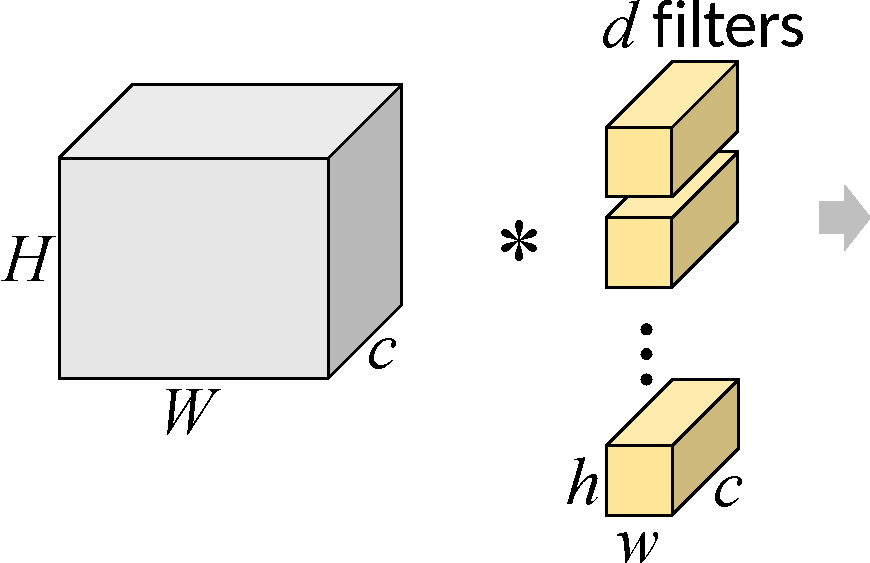
\includegraphics[width=0.29\textwidth, page=1, viewport = 0 0 440 300, clip=true]{layer}}
    \begin{tikzpicture}[ampersand replacement=\&]
\begin{scope}[]
\matrix[column sep=0em]{
	\node {
		\raisebox{-0.5\height}{\layer}
	};\&
	\node {
		\raisebox{-0.5\height}{\layer}
	};\&
	\node {
		\raisebox{-0.5\height}{\layer}
	};\&
	\node {
		\raisebox{-0.5\height}{$\cdots$}
	};\\
	};
	\end{scope}
	\end{tikzpicture}
	\caption[Vanishing gradients]{\textbf{Vanishing gradients.} For networks with many layers, even small deviations from a unit gradient are quickly geometrically magnified by propagation through all layers.}\label{fig:manylayers}
\end{figure}
Until relatively recently, pre-training was considered necessary for the feasibility of training deep neural networks\index{neural network}~\citep{hinton2006reducing}. The vanishing gradient problem was first addressed through better methods of random initialization which considered the geometric effect of propagating gradients through very \glspl{dnn}\index{DNN}. Without careful initialization, gradients can either surpass numerical representation (exploding gradients) or be reduced to close to zero (vanishing gradients). This effect is further exacerbated by the use of the softmax function at the end of the network, containing the exponential function.

For example, consider a deep network consisting of $L$ identical layers as shown in \cref{fig:manylayers}, and assume that our initialization results in the first pass through the network scaling the signal (i.e~gradients) by a factor of $\gls{beta}$ for each layer.

After propagating through $L$ layers, this becomes a scaling of $\gls{beta}^L$, exponentially magnifying the effect of the discrepancy. For example, the output of a trivial deep network, where each layer $l$ only maps the identity function, $f_{l}(x) = x$, with $L$ layers, and each layer is initialized such that the output response is scaled by $\gls{beta}$, will be:
%
\begin{equation}
\begin{aligned}
	f_L(x) & = (f_1 \gls{composition} f_2 \ldots \gls{composition} f_L) (x)\\
	& = x \, \prod^{L}_{l} \beta = x\, \beta^L,
\end{aligned}
\end{equation}
where $(f \gls{composition} g)(x)$ is the composition $f(g(x))$.
%
This problem has two distinct outcomes determined by the effective scaling of each layer's initialization $\gls{beta}$:
\[
\lim_{L\to\infty} f_L(x) = 
\begin{cases}
\infty & \text{if } \beta > 1, \text{ training loss \emph{diverges}}\\
0 & \text{if } \beta < 1, \text{ training loss \emph{stalls}}.
\end{cases}
\]
%
Thus we want a random initialization of layers such that $\gls{beta}\approx 1$ to minimize the `vanishing gradient' effect. For sigmoidal activation functions, such an initialization was proposed by \citet{glorot2010understanding}. For random Gaussian initialization, and given the number of outgoing/incoming connections to each neuron\index{neuron}, we can carefully choose the standard deviation $\gls{stddev}$ such that the expected value,

\begin{equation}
	\gls{expected}\left[\gls{beta}\right] = 1.
\end{equation}
In practice however, most networks have layers of different numbers of neurons\index{neuron}. In this case, since there are different numbers of incoming connections and outgoing connections for each neuron\index{neuron}, there are two possible initializations, one for the expected forward pass (response) scaling, and one for the backwards pass (gradient). As a compromise, \citet{glorot2010understanding} proposed to use the average number of outgoing and incoming connections to the neuron\index{neuron}:
%
\begin{equation}
\begin{aligned}
	\gls{stddev}_{\textrm{forwards}} &= \frac{1}{\sqrt{n_{\text{out}}}}\\
	\gls{stddev}_{\textrm{backwards}} &= \frac{1}{\sqrt{n_{\text{in}}}}\\
	\gls{stddev}_{\textrm{average}} &= \frac{1}{\sqrt{(n_{\text{out}} + n_{\text{in}})/2}}.
\end{aligned}
\end{equation}
%
For the more typically used rectified linear unit, a variation of this initialization was proposed by \citet{He2015b}:
%
\begin{equation}
\begin{aligned}
	\gls{stddev}_{\textrm{forwards}} &= \frac{2}{\sqrt{n_{\text{out}}}}\\
	\gls{stddev}_{\textrm{backwards}} &= \frac{2}{\sqrt{n_{\text{in}}}}\\
	\gls{stddev}_{\textrm{average}} &= \frac{2}{\sqrt{(n_{\text{out}} + n_{\text{in}})/2}}.
\end{aligned}
\end{equation}
%
\subsection{Batch Normalization}
Some network architectures are sufficiently complex, \ie networks with neurons\index{neuron} with drastically different number of outgoing/incoming connections, that even careful initialization will not prevent exploding/vanishing gradients. Instead, \citet{Ioffe2015} proposed a more direct approach of maintaining the desired zero-mean, unit Gaussian response distribution. Batch normalization\index{batch normalization|textbf} proposes to use batch statistics to whiten the responses of layers it is applied to during training.

%Batch normalization\index{batch normalization} maintains per-batch response statistics during training, and uses them to reshape the response distribution during training.
Full whitening (\ie de-correlating the responses) is prohibitively expensive however, instead batch normalization\index{batch normalization} calculates the mini-batch mean and variance, and prevents vanishing gradients by normalizing responses/gradients according to the batch statistics. Using batch-normalization during training can make a dramatic difference, in many cases networks that would previously not converge, will converge, and it can sometimes even speed up training.

The batch statistics calculated by batch normalization\index{batch normalization} are,
\begin{equation}
\begin{aligned}
    \mu_b &= \frac{1}{M} \sum^M_{i=0} x_i\\
    \gls{stddev}^2_b &= \frac{1}{M} \sum^M_{i=0}\\
    \gls{normx}_i &= \frac{x_i - \gls{mean}_b}{\sqrt{\gls{stddev}^2_b + \epsilon}},
\end{aligned}
\end{equation}
where for mini-batch $b$, $\gls{mean}_b$ is the mean, $\gls{stddev}^2_b$ is the variance, $\epsilon$ is for numerical stability, $\left\{x_0, \ldots, x_i, \ldots x_M\right\}$ are the mini-batch responses for a particular parameter of the layer, and $\gls{normx}_i$ is the normalized response for that parameter. 

Batch normalization\index{batch normalization} then uses these statistics, along with two parameters learned across mini-batches, $\gamma$ and $\beta$, to scale and shift the responses,
\begin{equation}    
    \gls{y}_i = \gamma \gls{normx}_i + \beta.
\end{equation}
%
Most state-of-the-art supervised \glspl{dnn}\index{DNN} now use batch normalization\index{batch normalization} along with the initialization, as presented in \cref{ssec:init}, to train.

\subsection{Dropout}
\citet{dropout,dropoutjmlr} introduced \emph{dropout}\index{dropout}, a method of preventing overfitting in large networks during training. The implementation of dropout is to, during training, effectively zero out a set of neurons, sampled randomly from each layer with a fixed probability $p$. At test time all the neurons are active, and to maintain the expected responses, a multiplicative factor of $p$ is used.

The mechanism of the effect of dropout is explained several different ways, and notably different explanations are given by \citet{dropout} and \citet{dropoutjmlr}\footnote{we have found some empirical evidence to suggest it is an optimization trick rather than a form of regularization, see \cref{dropoutasopttrick}.}. The explanation by \citet{dropout} is that dropout is a form of regularization by noise, preventing `co-adaption' of neurons (see \cref{pairablation}). The main explanation given by \citet{dropoutjmlr} is that dropout is a form of model integration, averaging over a large number of random `thinner' model architectures at training time in order to improve generalization. At training time however, averaging over all the models considered during training would  be extremely computationally expensive, since there are an exponential ($2^n$) number of possible models considered during training.

Empirically dropout improves generalization of networks with very large layers, in particular the large fully-connected layers to be found at the end of the \gls{alexnet} and \gls{vgg} architectures. It has less effect on models train with batch normalization\index{batch normalization} however, as observed by the authors~\citep{Ioffe2015}, and in practice is not used in more recent deep network architectures such as \gls{resnet}.

\section{Deep Neural Network Architectures}
An exhaustive list of every novel deep learning architecture would be infeasible, and outside the scope of this dissertation, however here we have made an effort to cover the recent architectures which have both inspired our work and formed the basis of many of our results.

\subsection{AlexNet}
Training \glspl{dnn}\index{DNN}, that is neural networks\index{neural network} with many (\ie two or more) hidden layers, had proven difficult due to the high computational complexity, and the so called `vanishing gradient' problem~\citep{bengio:ieeenn94}. \citet{Krizhevsky2012} showed that a deep \gls{cnn} (the specific architecture since referred to as AlexNet) trained on a very large dataset~\citep{ILSVRC2015}, with the appropriate initialization~\citep{Sutskever2013momentum}, weight decay\index{weight decay} \gls{relu} activation functions~\citep{conf/icml/NairH10} and dropout~\citep{Hinton2012} could beat state-of-the-art methods on large scale object class recognition methods, based on hand-crafted features, by a large margin. This single paper introduced or motivated many of the recent advances in training neural networks\index{neural network}, as covered in \cref{section:contemporary}.

AlexNet notably used training-time and test-time augmentation to achieve its state-of-the-art accuracy. During training random $224 \times 224$ crops of a $256 \times 256$ image are used, along with random mirroring of these crops. In addition \emph{relighting augmentation} is used, where the \gls{pca} components over all \gls{rgb} pixels in the image are used to perturb the ``brightness'' of the image, and give some robustness to photometric variations in the test images. At test time ``$10\times$ oversampling'' is used, that is for each $256\times 256$ test image, and its mirrored image, four corner and one centre crop are pushed through the network, and the prediction is simply the averaged over these 10 crops. Finally, for the best results reported (Top-5 error of 15.4\%), an \emph{ensemble} of 7 models is used, where the prediction is the average of all of these models. 

AlexNet uses two filter groups\index{filter groups} throughout most of the layers of the model in order to split computation and model parameters across two \gls{gpu}s, the motivation being that at the time \gls{gpu}s did not have enough memory to fit such a large model. The authors observed that the filters on each \gls{gpu} appeared to specialize to learn fundamentally different features regardless of initialization~\citep{Krizhevsky2012}. This interesting observation has mostly been ignored in subsequent networks where \gls{gpu} memory has increased enough that such a split of the network is not required, but the original observation is a fundamental motivation of our work.

%\subsection{\Glsfmttext{nin}}
\subsection{Network in Network}
\begin{figure}[tbp]
    \centering
    \includegraphics[width=0.95\textwidth, page=4]{groupfig}
    \caption[Low-dimensional embedding]{\textbf{\Glsfmttext{lde}.} Introduced in the \glsfmttext{nin} architecture, a \glsfmttext{lde} consists of learning a 1$\times$1 convolutional layer after a normal convolutional layer. The pairing of 1$\times$1 filters and a non-linearity (\ie \glsfmttext{relu}) can effectively learn a non-linear transformation into a different space. If $c_3 < c_2$, then a transformation into a lower-dimensional space is learned, and potentially a more compact embedding of the learned representation.}\label{fig:lowdimembedding}
\end{figure}
\afterpage{
\begin{landscape}
\begin{figure}[tbp]
\centering
\begin{tikzpicture}[ampersand replacement=\&]
\begin{scope}[]
\matrix[column sep=0em]{
	\node (1a) {
		\raisebox{-0.5\height}{\includegraphics[height=0.08\linewidth, page=15]{groupfig}}
	};\&
	\node (1b) {
		\raisebox{-0.5\height}{\includegraphics[height=0.11\linewidth, page=21]{groupfig}}
	};\&
	\node (1c) {
		\raisebox{-0.5\height}{\includegraphics[height=0.11\linewidth, page=22]{groupfig}}\hspace{1em}\raisebox{-0.5\height}{$\cdots$}
	};
	\\
	\draw node{{\footnotesize \textit{image}}/{\footnotesize \textit{conv1a}}};\&
	\draw node{\footnotesize \textit{conv1b}};\&
	\draw node{\footnotesize \textit{conv1c}};\\
	\node (2a) {
		\raisebox{-0.5\height}{$\cdots$}\hspace{1em}\raisebox{-0.5\height}{\includegraphics[height=0.09\linewidth, page=16]{groupfig}}
	};\&
	\node (2b) {
		\raisebox{-0.5\height}{\includegraphics[height=0.11\linewidth, page=8]{groupfig}}
	};\&
	\node (2c) {
		\raisebox{-0.5\height}{\includegraphics[height=0.11\linewidth, page=22]{groupfig}}\hspace{1em}\raisebox{-0.5\height}{$\cdots$}
	};\\
	\draw node{\footnotesize \textit{conv2a}};\&
	\draw node{\footnotesize \textit{conv2b}};\&
	\draw node{\footnotesize \textit{conv2c}};\\
	\node (3a) {
		\raisebox{-0.5\height}{$\cdots$}\hspace{1em}\raisebox{-0.5\height}{\includegraphics[height=0.09\linewidth, page=16]{groupfig}}
	};\&
	\node (3b) {
		\raisebox{-0.5\height}{\includegraphics[height=0.11\linewidth, page=8]{groupfig}}
	};\&
	\node (3c) {
		\raisebox{-0.5\height}{\includegraphics[height=0.11\linewidth, page=22]{groupfig}}\hspace{1em}\raisebox{-0.5\height}{$\cdots$}
	};\\
	\draw node{\footnotesize \textit{conv3a}};\&
	\draw node{\footnotesize \textit{conv3b}};\&
	\draw node{\footnotesize \textit{conv3c}};\\
	\&\node (3c) {
		\raisebox{-0.5\height}{$\cdots$}\hspace{1em}\raisebox{-0.5\height}{\includegraphics[height=0.09\linewidth, page=20]{groupfig}}
	};\\
	\&\draw node{\footnotesize \textit{\gls{gap}/output}};\\
};
\end{scope}
\end{tikzpicture}
\caption[\Glsfmttext{nin} architecture]{\textbf{\Glsfmttext{nin} Architecture.}  Coloured blocks represent the filters of each layer, grey blocks the intermediate \glsfmtplural{featuremap}\index{feature map} over which a layer's filters operate. \Glsfmttext{gap} is used at the end of the network.
}
\label{fig:networkinnetwork}
\end{figure}
\end{landscape}
}

\citet{Lin2013NiN} introduced \glsfmtfull{nin}, in which the main contribution was the use of so-called `micro networks', consisting of increased non-linearity between convolutions using 1$\times$1 convolutions. The authors claimed the extra non-linearities introduced allow the network to capture more complex functions. These 1$\times $1 convolutions, illustrated in \cref{fig:lowdimembedding}, have since been referred to as \acrlongpl{lde}\emph{low dimensional embeddings}. If the number of 1$\times$1 filters is lower than the number of normal convolutional filters, then the 1$\times$1 layer learns a non-linear transformation of the input \gls{featuremap}\index{feature map} into a smaller space, \ie a reduction in the number of filters by a mapping of a high-dimensional \gls{featuremap}\index{feature map} onto a lower-dimensional \gls{featuremap}\index{feature map}. This can be used to reduce the computation and parameters of convolutional layers significantly, while potentially learning a more compact and efficient representation. The full NiN architecture is shown in \cref{fig:networkinnetwork}.

\citet{Lin2013NiN} also introduced \emph{\gls{gap}\index{GAP|textbf}}, in which the spatial extents at the end of the convolutional layers (\ie pool5 for NiN/AlexNet) are aggregated such that there is only a single scalar output response for each filter in the pooled layer. After \gls{gap}\index{GAP} of a layer with $f$ filters/\glspl{featuremap}\index{feature map}, the input to the classification layer is simply a vector of $f$ responses, as illustrated in \cref{fig:networkinnetwork}. This reduces the parameters of the network dramatically since the majority of the parameters in the network are typically between the last convolutional layer and the fully-connected classification layer. Lin \etal showed that on \gls{cifar10} \gls{gap}\index{GAP} by itself achieved a lower error than having a fully-connected layer with dropout.

\subsection{VGG}
Since AlexNet, there have been many improvements to the state of the art on the \gls{ilsvrc} challenge, every one of which has been an improved \gls{cnn} architecture. One particular architecture that has lent itself to both high accuracy and being a natural extension of the original network has been that proposed by \citet{Simonyan2014verydeep} of the Visual Geometry Group (VGG) at Oxford. The primary contributions of the VGG network are
\begin{enumerate*}[label = (\textbf{\roman*})]
\item showing that very deep networks improve generalization, and
\item learning stacked small filters, \ie three 3$\times$3 convolutional layers is more computationally efficient than learning a single convolutional layer of 7$\times$7 filters, and also improves generalization
\end{enumerate*}.

VGG is an evolution of the AlexNet models, with the same number of max-pooling layers, however using very small convolutional filters ($3$$\times$$3$) in the convolutional layers, and many more of these convolutional layers between pooling, instead of the relatively large single-layers of convolutional filters in AlexNet ($7$$\times$$7$). In addition VGG uses small non-overlapping max-pooling ($2$$\times$$2$), and the \emph{fully convolutional trick} introduced by \citet{Sermanet2013overfeat} to do test-time oversampling more efficiently. VGG uses extensive training augmentation, extending the augmentation used in AlexNet~\citep{Krizhevsky2012} by adding scale augmentation, where crops are taken from images of different rescaled sizes. 

\subsection{Inception}\label{backgroundinception}
\begin{figure}
	\centering
	\includegraphics[width=0.7\textwidth, page=7]{sparsification}
	\caption[Illustration of the inception unit]{\textbf{\Glsfmttext{inception}\index{inception} unit.} The building block of the \glsfmttext{inception}/\glsfmttext{googlenet} architecture. Learns a limited number of large filters (7$\times$7, 5$\times$5), and a great number of small filters (3$\times$3, 1$\times$1), followed by a \gls{lde} (1$\times$1) layer.}\label{fig:inceptionunit}
\end{figure}
The winner of the \gls{ilsvrc}2014 challenge, as measured by classification accuracy, was the \emph{\gls{inception}\index{inception|textbf} architecture}, or \gls{googlenet}~\citep{Szegedy2014going}. The \gls{inception}\index{inception} architecture is particularly interesting, in that it was created explicitly to minimize computation and learn a more efficient representation. Although it uses the \gls{lde} of \gls{nin}, this is combined with a novel combination of filters of different spatial size, within what is called an \emph{\gls{inception}\index{inception} unit}, illustrated in \cref{fig:inceptionunit}.

The motivation of the architecture is that most of the important correlations in natural images are very localized, so much so that even 3$\times$3 filters can learn most of the important features, for example image gradients and edges --- as demonstrated by the VGG networks~\citep{Simonyan2014verydeep}. However, a few of the correlations are less localized, more complex, and better captured by 5$\times$5 or even 7$\times$7 filters. Instead of learning a lot of large and computationally expensive 7$\times$7 filters, the \gls{inception}\index{inception} unit learns mostly 1$\times$1, and 3$\times$3 filters, with fewer 5$\times$5 and even fewer 7$\times$7 filters. This represents a balance between representation and efficiency.

The authors explain this as learning `factorized' filters, however we disagree, and understand this architecture instead as learning a \emph{basis} for filters. Ignoring the non-linearity between the two layers in \cref{fig:inceptionunit}, heterogeneous filters on the same layer are concatenated into a single feature-map, which is then \emph{linearly combined} by the 1$\times$1 filters of the subsequent layer. This linear combination of smaller filters in order to represent a minimally parameterized, but effective filter of full-size (7$\times$7), is similar to representing a complex function as a parameterization of simpler basis functions.

\subsection{Residual Networks}\label{residualnetworks}
\begin{figure}[tbp]
\begin{subfigure}[T]{0.32\textwidth}
\centering
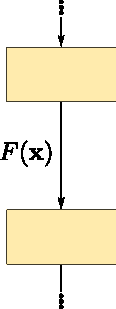
\includegraphics[height=0.215\textheight]{resnet-1}
\caption{}\label{fig:resnet-1}
\end{subfigure}
~
\begin{subfigure}[T]{0.32\textwidth}
\centering
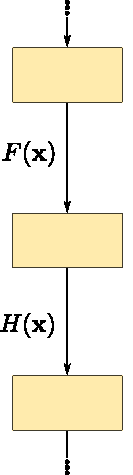
\includegraphics[height=0.33\textheight]{resnet-2}
\caption{}\label{fig:resnet-2}
\end{subfigure}
~
\begin{subfigure}[T]{0.32\textwidth}
\centering
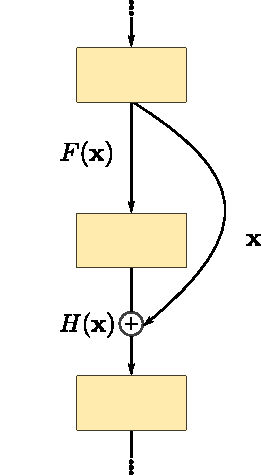
\includegraphics[height=0.33\textheight]{resnet-3}
\caption{}\label{fig:resnet-3}
\end{subfigure}
\caption[Residual networks]{\textbf{Residual networks.} \subref{fig:resnet-1} A convolutional network, where the mapping between the final two layers is $F(\gls{vectorx})$, \subref{fig:resnet-2} learning an additional layer with the mapping $H(\gls{vectorx})$, and \subref{fig:resnet-3} learning an additional residual layer with the mapping $H(\gls{vectorx})+\gls{vectorx}$.}
\label{fig:resnet}
\end{figure}
\citet{He2015} introduced residual networks\index{ResNet|textbf}, which provide an important insight on a problem with the training of very deep networks. While deeper networks have been found to improve generalization, especially with large datasets; at a sufficiently large depth training becomes difficult, even with batch normalization\index{batch normalization} and the correct initialization, and generalization begins to level off, or even decline.

The important insight of \citet{He2015} into this problem can be summarized in \cref{fig:resnet}. Having trained a deep network with good generalization (\ie \cref{fig:resnet-1}), with $N$ layers, a training loss of $\gls{L}_1$ is observed. On adding a single-layer to the otherwise identical deep network architecture (\ie \cref{fig:resnet-2}), and re-training from random initialization, the new training loss of the network with $N+1$ layers is found to be $\gls{L}_2 > \gls{L}_1$, \ie the training loss has increased.

Yet from an optimization standpoint it is not clear why this should be so. We can observe that there is a trivial set of parameters defining a transformation that will maintain the training loss of the shallower network, \ie $\gls{L}_1 = \gls{L}_1$ --- that is the identity transformation $H(\gls{vectorx})=x$. 

\citet{He2015} proposed that in order to aid the optimization, a \emph{residual connection} (as in \cref{fig:resnet-3}) is added to the convolutional layers, allowing the trivial identity solution to be easily learned. This residual connection can be thought of as a shortcut, bypassing the previous layer. Assuming our desired, but difficult to optimize, mapping from one layer to the next is $H(x)$, the residual function learned is simply:
\begin{equation}
	H(x) + x.
\end{equation}
%
In practice these residual layers greatly help the training of very deep networks, and have pushed state-of-the-art accuracy in many datasets. All current state-of-the-art models for image classification use residual layers.

% \section{Decision Forests}
% \subsection{Decision Trees}
% Decision trees have played a part in statistics, and machine learning, for a long time. They have their roots in classification trees, human generated versions of which have been commonly used for hierarchical classification of animal and plant species. As such they are conceptually amongst the simplest classification methods to understand. 

% In machine learning we are interested in automatically learning classifiers from training data. However, despite the simplicity of decision trees, in general learning an optimal decision tree for a given training set has been shown to be NP-hard~\citep{journals/iandc/HancockJLT96}. For this reason greedy training algorithms are used to train and grow trees from training data, based on various heuristics, typically measures of entropy or information gain at split nodes~\citep{breiman84}. 

% Like nearest neighbours, deep decision trees can easily achieve perfect training set accuracy, but do not generalize well. 

% \subsection{Random Forests/Decision Forests}
% Interest in decision trees has recently been revived in machine learning since new methods for training decision trees can result in good generalization. In particular Decision Forests (Random Forests)~\citep{journals/neco/AmitG97,breiman2001random}, were introduced as an ensemble method for decision trees.

% Random forests exploit two forms of the bagging method~\citep{breiman1996bagging}. In a random forest composed of $N$ decision trees, a different random subset of the training set is used to train each of the individual decision trees. In a further bagging step, a subset of the input features are randomly selected to train each decision tree. After training the decision trees, regression predictions are made from the average of the individual decision tree predictions,

% \begin{equation}
% 	f(x) = \frac{1}{N} \sum_{i=1}^{N} f_i(x),
% \end{equation}

% where $f$ is the random forest prediction, $x$ is the input, and $f_i$ are the individual decision trees.

% \section{The relationship between Decision Forests and Neural Networks}
% There has been work in the past exploring the relationship between decision forests and neural networks\index{neural network}. Although this work has identified that neural networks\index{neural network} are a generalization of decision forests, it focused on exploiting tree training towards either the initialization or training of neural networks\index{neural network}, rather than creating hybrid models exploiting the conditional computation in random forests, while preserving end-to-end training found in state-of-the-art deep neural networks\index{neural network}.


% \subsection{Entropy Nets}
% The relationship between decision forests and neural networks\index{neural network} was first described by \citet{Sethi1990}, the primary intuition of which is that the decision boundaries which are explicitly expressed in a decision tree can also be represented by a three-layer neural network\index{neural network}, where the decision nodes of the tree are on the first layer, the leaf nodes on the second layer.

% \subsection{Casting Random Forests as Artificial Neural Networks}
% More recently this relationship was rediscovered~\citep{Welbl2014casting}, in a very similar manner a method of initializing a neural network\index{neural network} with a trained Random Forest in described. The primary motivation of this is to use the trained random forest as a good initialization of a neural network\index{neural network} in order to avoid the neural network\index{neural network} from overfitting during stochastic gradient descent.

\end{document}
